%----------------------------------------------------------------------------------------
%    PACKAGES AND THEMES
%----------------------------------------------------------------------------------------

\documentclass[aspectratio=169,xcolor=dvipsnames]{beamer}
\usetheme{SimplePlus}
\usepackage{tikz}  % 用于绘图
\usepackage{amsmath}  % 更好的数学公式支持
\usepackage{amssymb}  % 数学符号
\usepackage{tcolorbox}
\usetikzlibrary{shapes, arrows, positioning, calc}  % TikZ库
\usepackage{bm}
\usepackage{xcolor}
\usetikzlibrary{decorations.pathm, patterns}
\usepackage{hyperref}
\usepackage{graphicx} % Allows including images
\usepackage{booktabs, tabularray} % Allows the use of \toprule, \midrule and \bottomrule in tables
\graphicspath{{figures/}}

%----------------------------------------------------------------------------------------
%    TITLE PAGE
%----------------------------------------------------------------------------------------
\title{曲梁结构免自锁有限元无网格法\\及其在屈曲分析中的应用}

\author{汇报人：何祖彦}

% 新增指导老师信息
\newcommand{\advisorname}{指导老师：吴俊超} % 请在此处填入指导老师的姓名

% 自定义标题页模板，包含指导老师信息和校徽
\setbeamertemplate{title page}{%
 % 在左上角添加文字
    \begin{flushleft}
        \vspace{0.5em}
        \hspace{0.5em}
        \begin{minipage}[t]{0.8\textwidth}
            \raggedright
            \usebeamerfont{institute}
            \color{DarkBlue}
            \textbf{土木工程学院2024级开题汇报}\\
        \end{minipage}
    \end{flushleft}
    \vspace{0.1em} % 调整顶部间距为logo留出空间
    
    % 在顶部添加华侨大学校徽
    \begin{center}
        
\includegraphics[width=2.5cm]{hqu2.png} % 调整校徽大小
        \vspace{0.3em}
    \end{center}
    
    \begingroup
    \centering
    % ------------------------
    \begin{beamercolorbox}[sep=1pt,center]{title}
        \usebeamerfont{title}\inserttitle\par%
        \ifx\insertsubtitle\@empty%
        \else%
        \vskip0.25em%
        {\usebeamerfont{subtitle}\usebeamercolor[fg]{subtitle}\insertsubtitle\par}%
        \fi%
    \end{beamercolorbox}%
    \vskip1em\par
    % ------------------------
    \begin{beamercolorbox}[sep=3pt,center]{author}
        \usebeamerfont{author}\insertauthor
    \end{beamercolorbox}
    % 添加指导老师信息，与作者名字保持1pt间距
    \vskip1pt
    \begin{beamercolorbox}[sep=5pt,center]{author}
        \usebeamerfont{author}\advisorname
    \end{beamercolorbox}
    \vskip0.5em
    % ------------------------
    \begin{beamercolorbox}[sep=3pt,center]{date}
        \usebeamerfont{date}\insertdate
    \end{beamercolorbox}\vskip0.5em
    % ------------------------
    {\usebeamercolor[fg]{titlegraphic}\inserttitlegraphic\par}
    \endgroup
    \vfill
}

\date{2025年12月12日} % Date, can be changed to a custom date

%----------------------------------------------------------------------------------------
%    PRESENTATION SLIDES
%----------------------------------------------------------------------------------------

\begin{document}

\begin{frame}
    % Print the title page as the first slide
    \titlepage
\end{frame}

\begin{frame}{目录}
    % Throughout your presentation, if you choose to use \section{} and \subsection{} commands, these will automatically be printed on this slide as an overview of your presentation
    \tableofcontents
\end{frame}

\section{研究背景}

% 在您的 LaTeX 文档中合适位置添加以下代码
\begin{frame}{研究背景}

\begin{center}
% 并排插入两张图片
\begin{minipage}[t]{0.48\linewidth}
    \centering
    \includegraphics[width=\linewidth]{16.jpg} \\[0.5em]
\end{minipage}
\hfill
\begin{minipage}[t]{0.48\linewidth}
    \centering
    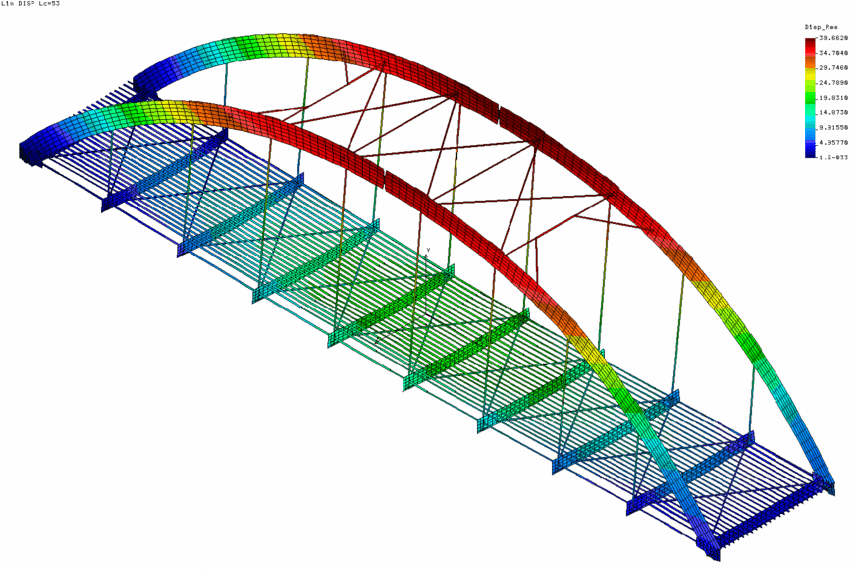
\includegraphics[width=\linewidth]{31.png} \\[0.5em]
\end{minipage}
\end{center}

\vspace{1em}

\begin{center}
\textbf{主要研究对象为考虑横向剪切应变的曲梁结构}
\end{center}

\end{frame}

\begin{frame}{研究背景}

\begin{columns}[T,totalwidth=\textwidth]
\flushleft
%======================== 左侧 ============================
\column{0.52\textwidth}
\textbf{弯矩与应力} \\
\vspace{0.5em}
$M_b = EI \kappa$ , $ N = EA \varepsilon$ , $Q = kGA \gamma $\\

\textbf{曲率与应变} \\
\vspace{0.5em}
$\kappa = \varphi_{,s}$ , $ \varepsilon = u_{,s} - \dfrac{w}{R} $ , $\gamma = w_{,s} + \dfrac{u}{R} - \varphi $\\

\vspace{0.5em}
\textbf{抗剪和抗弯}\\
\vspace{0.5em}
$EI = \dfrac{Ebh^3}{12} \propto h^3$ \\[0.25em]
$ kGA = kG(bh) \propto h$\\[0.25em]
$EA = E(bh) \propto h$\\
\textbf{剪切自锁}\\
\vspace{0.5em}
$h \to 0$  , $EI \ll (EA , kGA)$ , $(\varepsilon,\gamma) \to 0$

%======================== 右侧 ============================
\column{0.48\textwidth}
\flushleft
\vspace{-1.3em}
\textbf{屈曲理论}

\vspace{0.5em}
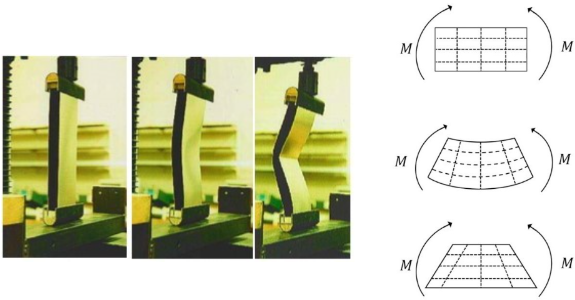
\includegraphics[width=7cm,height=6cm,keepaspectratio]{m5.png}

临界载荷 $P_{\text{cr}} = \dfrac{\pi^{2} EI}{(KL)^{2}}$

\end{columns}

\end{frame}

\begin{frame}{研究背景}

\begin{columns}[t]
\column{0.35\textwidth}
\centering\textbf{缩减积分}\\
\raggedright
\vspace{1em}
\quad \quad\quad \quad \quad \quad \quad \quad \quad  \textbf{积分}\\
\quad \quad$EI = \dfrac{Ebh^3}{12}$ \quad \quad{\huge→} \\[1em]
\quad \quad$kGA = kG(bh)$\\
\vspace{4.3em}

\quad \quad\quad \quad \quad \quad \quad \quad \quad \textbf{积分}\\
\quad \quad$EA = E(bh) $ \quad \quad {\huge→} \\
\vspace{0.2em}
\begin{figure}[ht] 

\includegraphics[width=0.07\linewidth]{m7.png} \quad \textbf{积分点}
\end{figure}

%------------------------
\column{0.3\textwidth}
\begin{figure}[ht] 
\centering % 确保图片在figure内水平居中
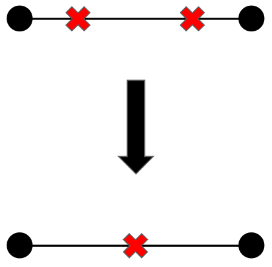
\includegraphics[width=4.5cm, height=4.5cm\linewidth]{m6.png}
\end{figure}
\column{0.35\textwidth}
%------------------------
\centering\textbf{混合离散}\\
\vspace{1em}
\textbf{离散} \quad \quad \quad \quad \quad \quad \quad \quad \quad \quad \quad\\
{\huge←} \quad $u^h(x) = \sum_{I=1}^{n_u} N_I^u(x) \, d_I $ \quad \quad\\
\vspace{1em}
\quad \quad $w^h(x) = \sum_{I=1}^{n_w} M_I^w(x) \, e_I $\\[1em]
\quad \quad $\psi(x) = \sum_{I=1}^{n_\psi} P_I^\psi(x) \, \psi_I $ \\
\vspace{1em}

$M_b = EI \kappa$\quad \quad \quad\\[0.5em]
$N = EA \varepsilon $\quad \quad \quad\\[0.5em]
\vspace{-1.5em}
\textbf{离散} \quad \quad \quad \quad \quad \quad \quad \quad \quad \quad \quad \\
{\huge←}\quad $Q = kGA\gamma $\quad \quad \quad \quad

\begin{figure}[ht] 

\includegraphics[width=0.07\linewidth]{m7.png} \quad \textbf{自由度}
\end{figure}

\end{columns}
\end{frame}

\begin{frame}{研究背景}
\textbf{目前存在问题：}
\vspace{3em}
\begin{enumerate}
\item 目前的有限元都只考虑膜应变和剪切应变，忽略了膜应力和剪切应力\\[3em] 
\item $u,w,Q,N$自由度目前匹配情况尚未清楚，无法 LBB 稳定性建立联系\\[3em]
\item 目前的有限元方法都基于单元，无法对约束比进行调整。
\end{enumerate}
\end{frame}


\section{研究方案} 

\begin{frame}{研究方案}
\begin{center}
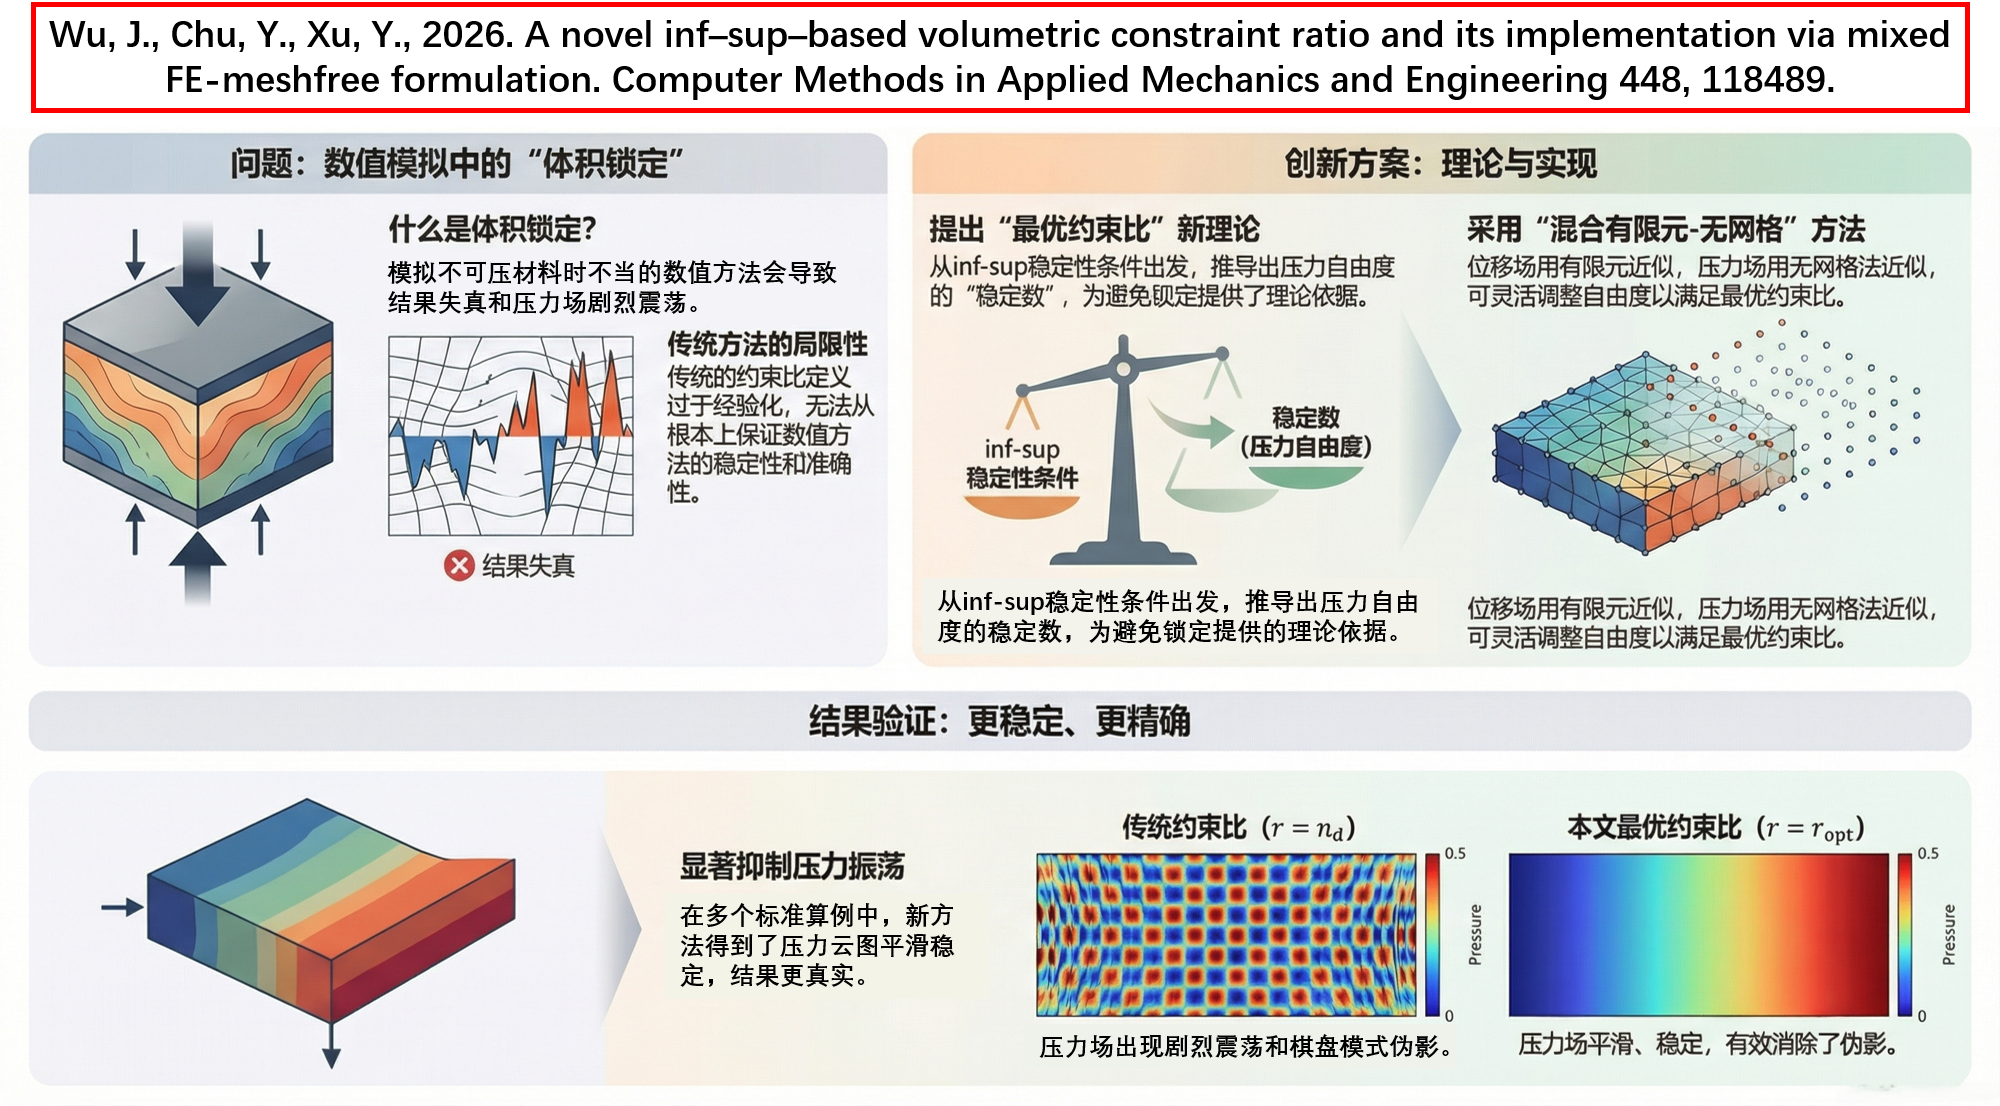
\includegraphics[width=13.2cm]{m13.png} % 調整圖片大小
\end{center}
\end{frame}

\begin{frame}{研究方案}
\textbf{伽辽金弱形式}
\begin{align*}
a(\delta \varphi,\varphi) + b_{\varphi}(\delta \varphi,Q) &= f_{\varphi}(\delta \varphi) \\
\textcolor{blue}{b_{u}(\delta u,\{N,Q\}) &= f_{u}(\delta u)} \\
\textcolor{blue}{b_{w}(\delta w,\{N,Q\}) &= f_{w}(\delta w)} \\
\textcolor{red}{b_{N}(\delta N,\varepsilon) &= f_{N}(\delta N)} \\
\textcolor{red}{b_{Q}(\delta Q,\gamma) &= f_{Q}(\delta Q)}
\end{align*}

\begin{columns}[onlytextwidth,T]
\begin{column}{0.4\textwidth}
    \centering
    \textbf{\textcolor{blue}{薄膜应力和剪切应力约束}}
\\[-0.75em]
\[
\begin{aligned}
\textcolor{blue}{\inf_{u_h\in U_h} \sup_{ q_h \in Q_h} \frac{\vert b_{u}(\delta u,\{N,Q\})\vert}{\Vert u_h\Vert_U \Vert  N_h,Q_h \Vert_Q} \ge \beta_{N,Q}}\\[1em]
\textcolor{blue}{\inf_{w_h\in W_h} \sup_{ q_h \in Q_h} \frac{\vert b_{w}(\delta w,\{N,Q\})\vert}{\Vert w_h\Vert_W \Vert  N_h,Q_h \Vert_Q} \ge \beta_{N,Q}}
\end{aligned}
\]
\end{column}


\begin{column}{0.2\textwidth}
    \vspace{2em}
    \centering
    dim($u$)\\
    dim($w$)\\
    dim($N$)\\
    dim($Q$)\\
$\Leftrightarrow$
\end{column}
\begin{column}{0.4\textwidth}
    \centering
    \textbf{\textcolor{red}{薄膜应变和剪切应变约束}}
    \\[-0.75em]
\[
\begin{aligned}
\textcolor{red}{\inf_{ N_h \in N_h} \sup_{ N_h \in N_h \times \Phi_h}
\frac{\vert b_{N}(\delta N,\varepsilon) \vert}{\Vert  N_h \Vert_{N\times \Phi} \Vert  \varepsilon \Vert_Q } \ge \beta_{\varepsilon}}\\[1em]
\textcolor{red}{\inf_{ Q_h \in Q_h} \sup_{ Q_h \in Q_h \times \Phi_h}
\frac{\vert b_{Q}(\delta Q,\gamma) \vert}{\Vert  Q_h \Vert_{Q\times \Phi} \Vert  \gamma \Vert_Q } \ge \beta_{\gamma}}
\end{aligned}
\]
\end{column}

\end{columns}
\end{frame}


\begin{frame}{研究方案}
\begin{columns}[onlytextwidth,T]
% 右侧栏：美化流程图
\begin{column}{0.5\textwidth}
    \vspace{-0.5em}
    \textbf{一维有限元}
        \begin{center}
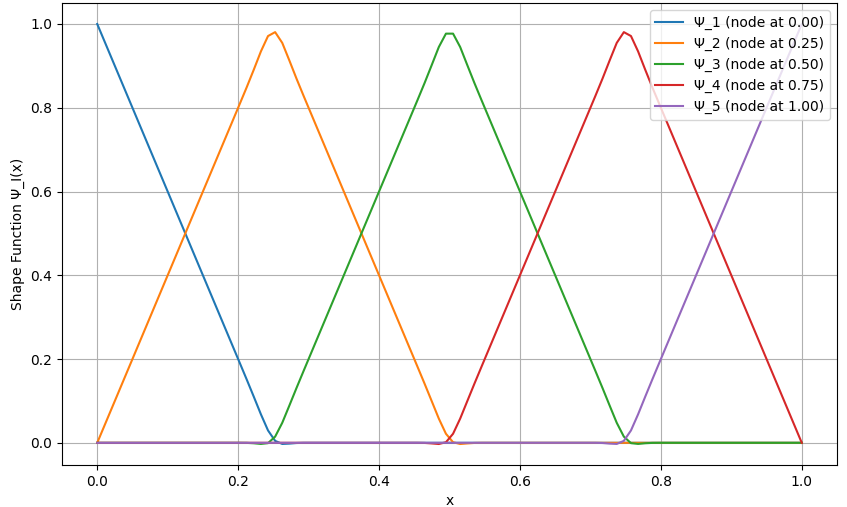
\includegraphics[width=6cm]{f8.png} % 調整圖片大小
\end{center}
\textbf{无网格径向基函数(RK)形函数的优势}
\item 便于布置无网格节点 $\Rightarrow$ \textbf{可任意调整约束比}
\item 全局光滑性 $\Rightarrow$ \textbf{便于数值实现}
\item 一致性条件 $\Rightarrow$ \textbf{保证计算精度}
\end{column}

% 左侧栏：问题与解决方案
\begin{column}{0.5\textwidth}
\vspace{-0.5em}  % 调整顶部间距
\textbf{一维无网格}
\begin{center}
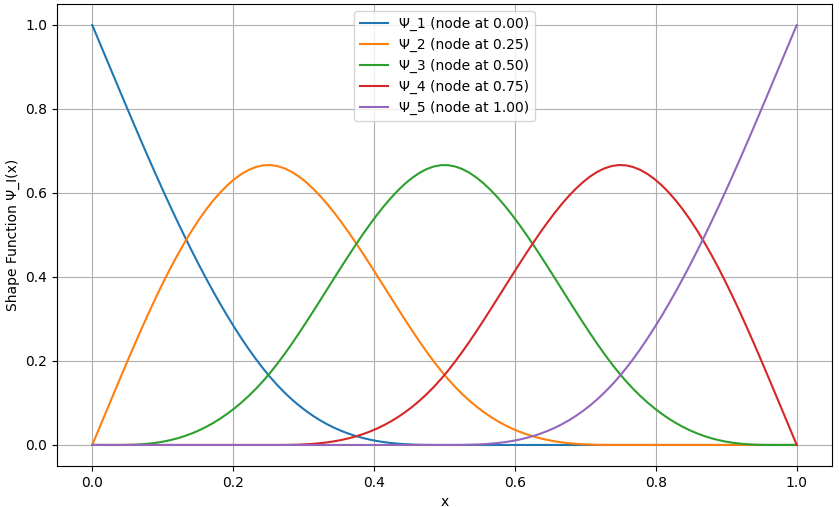
\includegraphics[width=6cm]{f7.png} % 調整圖片大小
\end{center}
\end{column}

\end{columns}

\end{frame}

\section{研究內容}

\begin{frame}{研究内容}
    \begin{columns}[c]
        \column{0.3\textwidth}
 \begin{center}
            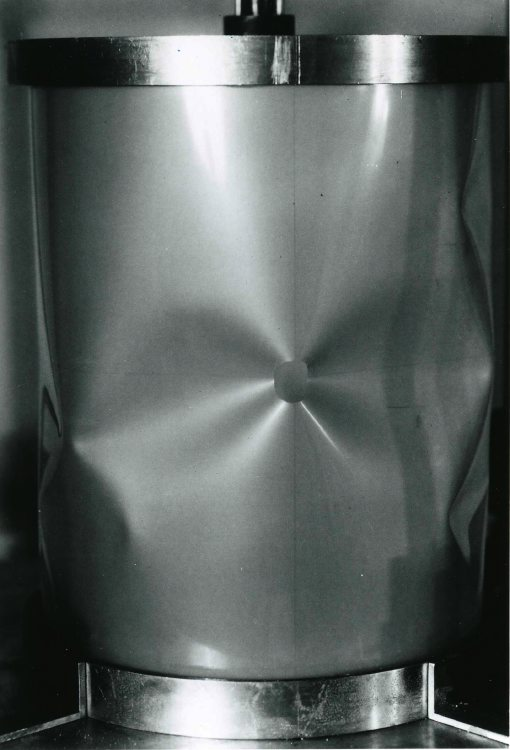
\includegraphics[width=4cm]{f11.jpg} % 調整圖片大小
        \end{center}

        \column{0.3\textwidth}
         \begin{center}
            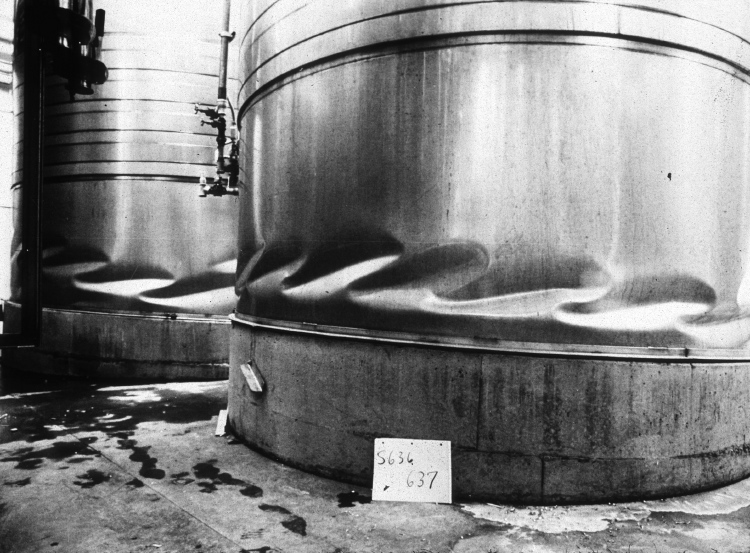
\includegraphics[width=5cm]{f12.jpg} % 調整圖片大小
        \end{center}

        \column{0.3\textwidth}
        \begin{center}
            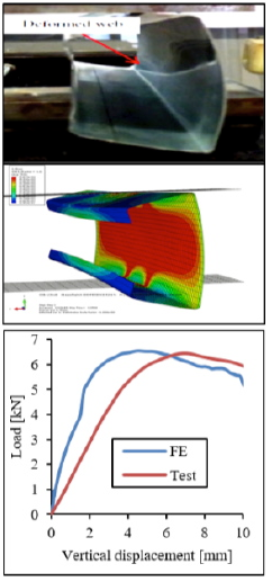
\includegraphics[width=3.2cm]{m12.png} % 調整圖片大小
        \end{center}
    \end{columns}
\end{frame}

\section{进度安排}

\begin{frame}{研究进度}
    \vspace{0.2cm} % 减少顶部空白
% 使用 tabularray 包创建美观的表格
\centering
\begin{tblr}{
    width = 0.95\linewidth,
    colspec = {X[1,l] X[2.3,l] X[0.8,c]},  %：移除逗號
    row{1} = {font=\bfseries, c, },  % 添加表頭背景色
    row{2-Z} = {rowsep=5pt},
    row{6} = {font=\normalsize},
    cell{7}{1} = {c=3}{r},
    hline{1,2,8} = {1pt}, % 顶部、表头下、底部的线
    % hline{3,4,5,7} = {0.5pt, solid}, % 行之间的细线
    vlines = {0pt}, % 不显示垂直线
}
\textbf{時間} & \textbf{研究內容} & \textbf{進度情況} \\
2025.7-2025.12 & 推导剪切应力和薄膜应力自锁的LBB稳定性条件 & \scalebox{2}{$\circ$} \\
2026.1-2026.2 & 进行Timoshenko曲梁的混合离散分析 & \\
2026.3-2026.9 & 曲梁结构免自锁在屈曲分析中的应用 &  \\
2026.10-2026.12 & 整理成果并完成论文初稿撰写 &\\
2027.1-2027.3 & 进一步修改完善论文，形成并提交论文终稿 &  \\
\scalebox{2}{$\bullet$} 已完成 \quad \scalebox{2}{$\circ$} 正在進行 & & \\
\end{tblr}

% 在表格和图例之间添加弹性空间
\vspace*{\fill}

% 在页面底部添加2em的固定距离
\vspace{2em}
\end{frame}

\begin{frame}
    \Huge{\centerline{\textbf{请各位老师批评指正！}}}
\end{frame}

\end{document}